% Options for packages loaded elsewhere
% Options for packages loaded elsewhere
\PassOptionsToPackage{unicode}{hyperref}
\PassOptionsToPackage{hyphens}{url}
\PassOptionsToPackage{dvipsnames,svgnames,x11names}{xcolor}
%
\documentclass[
]{article}
\usepackage{xcolor}
\usepackage[top=0.75in,left=0.75in,bottom=0.75in,right=0.75in]{geometry}
\usepackage{amsmath,amssymb}
\setcounter{secnumdepth}{5}
\usepackage{iftex}
\ifPDFTeX
  \usepackage[T1]{fontenc}
  \usepackage[utf8]{inputenc}
  \usepackage{textcomp} % provide euro and other symbols
\else % if luatex or xetex
  \usepackage{unicode-math} % this also loads fontspec
  \defaultfontfeatures{Scale=MatchLowercase}
  \defaultfontfeatures[\rmfamily]{Ligatures=TeX,Scale=1}
\fi
\usepackage{lmodern}
\ifPDFTeX\else
  % xetex/luatex font selection
\fi
% Use upquote if available, for straight quotes in verbatim environments
\IfFileExists{upquote.sty}{\usepackage{upquote}}{}
\IfFileExists{microtype.sty}{% use microtype if available
  \usepackage[]{microtype}
  \UseMicrotypeSet[protrusion]{basicmath} % disable protrusion for tt fonts
}{}
\makeatletter
\@ifundefined{KOMAClassName}{% if non-KOMA class
  \IfFileExists{parskip.sty}{%
    \usepackage{parskip}
  }{% else
    \setlength{\parindent}{0pt}
    \setlength{\parskip}{6pt plus 2pt minus 1pt}}
}{% if KOMA class
  \KOMAoptions{parskip=half}}
\makeatother
% Make \paragraph and \subparagraph free-standing
\makeatletter
\ifx\paragraph\undefined\else
  \let\oldparagraph\paragraph
  \renewcommand{\paragraph}{
    \@ifstar
      \xxxParagraphStar
      \xxxParagraphNoStar
  }
  \newcommand{\xxxParagraphStar}[1]{\oldparagraph*{#1}\mbox{}}
  \newcommand{\xxxParagraphNoStar}[1]{\oldparagraph{#1}\mbox{}}
\fi
\ifx\subparagraph\undefined\else
  \let\oldsubparagraph\subparagraph
  \renewcommand{\subparagraph}{
    \@ifstar
      \xxxSubParagraphStar
      \xxxSubParagraphNoStar
  }
  \newcommand{\xxxSubParagraphStar}[1]{\oldsubparagraph*{#1}\mbox{}}
  \newcommand{\xxxSubParagraphNoStar}[1]{\oldsubparagraph{#1}\mbox{}}
\fi
\makeatother

\usepackage{color}
\usepackage{fancyvrb}
\newcommand{\VerbBar}{|}
\newcommand{\VERB}{\Verb[commandchars=\\\{\}]}
\DefineVerbatimEnvironment{Highlighting}{Verbatim}{commandchars=\\\{\}}
% Add ',fontsize=\small' for more characters per line
\usepackage{framed}
\definecolor{shadecolor}{RGB}{241,243,245}
\newenvironment{Shaded}{\begin{snugshade}}{\end{snugshade}}
\newcommand{\AlertTok}[1]{\textcolor[rgb]{0.68,0.00,0.00}{#1}}
\newcommand{\AnnotationTok}[1]{\textcolor[rgb]{0.37,0.37,0.37}{#1}}
\newcommand{\AttributeTok}[1]{\textcolor[rgb]{0.40,0.45,0.13}{#1}}
\newcommand{\BaseNTok}[1]{\textcolor[rgb]{0.68,0.00,0.00}{#1}}
\newcommand{\BuiltInTok}[1]{\textcolor[rgb]{0.00,0.23,0.31}{#1}}
\newcommand{\CharTok}[1]{\textcolor[rgb]{0.13,0.47,0.30}{#1}}
\newcommand{\CommentTok}[1]{\textcolor[rgb]{0.37,0.37,0.37}{#1}}
\newcommand{\CommentVarTok}[1]{\textcolor[rgb]{0.37,0.37,0.37}{\textit{#1}}}
\newcommand{\ConstantTok}[1]{\textcolor[rgb]{0.56,0.35,0.01}{#1}}
\newcommand{\ControlFlowTok}[1]{\textcolor[rgb]{0.00,0.23,0.31}{\textbf{#1}}}
\newcommand{\DataTypeTok}[1]{\textcolor[rgb]{0.68,0.00,0.00}{#1}}
\newcommand{\DecValTok}[1]{\textcolor[rgb]{0.68,0.00,0.00}{#1}}
\newcommand{\DocumentationTok}[1]{\textcolor[rgb]{0.37,0.37,0.37}{\textit{#1}}}
\newcommand{\ErrorTok}[1]{\textcolor[rgb]{0.68,0.00,0.00}{#1}}
\newcommand{\ExtensionTok}[1]{\textcolor[rgb]{0.00,0.23,0.31}{#1}}
\newcommand{\FloatTok}[1]{\textcolor[rgb]{0.68,0.00,0.00}{#1}}
\newcommand{\FunctionTok}[1]{\textcolor[rgb]{0.28,0.35,0.67}{#1}}
\newcommand{\ImportTok}[1]{\textcolor[rgb]{0.00,0.46,0.62}{#1}}
\newcommand{\InformationTok}[1]{\textcolor[rgb]{0.37,0.37,0.37}{#1}}
\newcommand{\KeywordTok}[1]{\textcolor[rgb]{0.00,0.23,0.31}{\textbf{#1}}}
\newcommand{\NormalTok}[1]{\textcolor[rgb]{0.00,0.23,0.31}{#1}}
\newcommand{\OperatorTok}[1]{\textcolor[rgb]{0.37,0.37,0.37}{#1}}
\newcommand{\OtherTok}[1]{\textcolor[rgb]{0.00,0.23,0.31}{#1}}
\newcommand{\PreprocessorTok}[1]{\textcolor[rgb]{0.68,0.00,0.00}{#1}}
\newcommand{\RegionMarkerTok}[1]{\textcolor[rgb]{0.00,0.23,0.31}{#1}}
\newcommand{\SpecialCharTok}[1]{\textcolor[rgb]{0.37,0.37,0.37}{#1}}
\newcommand{\SpecialStringTok}[1]{\textcolor[rgb]{0.13,0.47,0.30}{#1}}
\newcommand{\StringTok}[1]{\textcolor[rgb]{0.13,0.47,0.30}{#1}}
\newcommand{\VariableTok}[1]{\textcolor[rgb]{0.07,0.07,0.07}{#1}}
\newcommand{\VerbatimStringTok}[1]{\textcolor[rgb]{0.13,0.47,0.30}{#1}}
\newcommand{\WarningTok}[1]{\textcolor[rgb]{0.37,0.37,0.37}{\textit{#1}}}

\usepackage{longtable,booktabs,array}
\usepackage{calc} % for calculating minipage widths
% Correct order of tables after \paragraph or \subparagraph
\usepackage{etoolbox}
\makeatletter
\patchcmd\longtable{\par}{\if@noskipsec\mbox{}\fi\par}{}{}
\makeatother
% Allow footnotes in longtable head/foot
\IfFileExists{footnotehyper.sty}{\usepackage{footnotehyper}}{\usepackage{footnote}}
\makesavenoteenv{longtable}
\usepackage{graphicx}
\makeatletter
\newsavebox\pandoc@box
\newcommand*\pandocbounded[1]{% scales image to fit in text height/width
  \sbox\pandoc@box{#1}%
  \Gscale@div\@tempa{\textheight}{\dimexpr\ht\pandoc@box+\dp\pandoc@box\relax}%
  \Gscale@div\@tempb{\linewidth}{\wd\pandoc@box}%
  \ifdim\@tempb\p@<\@tempa\p@\let\@tempa\@tempb\fi% select the smaller of both
  \ifdim\@tempa\p@<\p@\scalebox{\@tempa}{\usebox\pandoc@box}%
  \else\usebox{\pandoc@box}%
  \fi%
}
% Set default figure placement to htbp
\def\fps@figure{htbp}
\makeatother





\setlength{\emergencystretch}{3em} % prevent overfull lines

\providecommand{\tightlist}{%
  \setlength{\itemsep}{0pt}\setlength{\parskip}{0pt}}



 


\makeatletter
\@ifpackageloaded{caption}{}{\usepackage{caption}}
\AtBeginDocument{%
\ifdefined\contentsname
  \renewcommand*\contentsname{Table of contents}
\else
  \newcommand\contentsname{Table of contents}
\fi
\ifdefined\listfigurename
  \renewcommand*\listfigurename{List of Figures}
\else
  \newcommand\listfigurename{List of Figures}
\fi
\ifdefined\listtablename
  \renewcommand*\listtablename{List of Tables}
\else
  \newcommand\listtablename{List of Tables}
\fi
\ifdefined\figurename
  \renewcommand*\figurename{Figure}
\else
  \newcommand\figurename{Figure}
\fi
\ifdefined\tablename
  \renewcommand*\tablename{Table}
\else
  \newcommand\tablename{Table}
\fi
}
\@ifpackageloaded{float}{}{\usepackage{float}}
\floatstyle{ruled}
\@ifundefined{c@chapter}{\newfloat{codelisting}{h}{lop}}{\newfloat{codelisting}{h}{lop}[chapter]}
\floatname{codelisting}{Listing}
\newcommand*\listoflistings{\listof{codelisting}{List of Listings}}
\makeatother
\makeatletter
\makeatother
\makeatletter
\@ifpackageloaded{caption}{}{\usepackage{caption}}
\@ifpackageloaded{subcaption}{}{\usepackage{subcaption}}
\makeatother
\usepackage{bookmark}
\IfFileExists{xurl.sty}{\usepackage{xurl}}{} % add URL line breaks if available
\urlstyle{same}
\hypersetup{
  pdftitle={Lab Ten -- Point Estimation},
  colorlinks=true,
  linkcolor={blue},
  filecolor={Maroon},
  citecolor={Blue},
  urlcolor={Blue},
  pdfcreator={LaTeX via pandoc}}


\title{Lab Ten -- Point Estimation}
\author{}
\date{}
\begin{document}
\maketitle


\normalsize

\normalsize

\textbf{Tips}

\begin{itemize}
\tightlist
\item
  Complete the tasks below. Make sure to start your solutions in on a
  new line that starts with ``\textbf{Solution}:''.
\item
  Make sure to use the Quarto Cheatsheet. This will make completing and
  writing up the lab \emph{much} easier.
\item
  Make sure to use ``enter'' to make your code readable, so it doesn't
  run off the page. I switched the Quarto document to automatically
  render to .pdf, so you can see what you're submitting by default. You
  can switch back for the highlighting by moving the html block above
  the pdf block in the YAML header.
\item
  Don't forget that you can copy-and-paste code when you're doing
  something similar as we did in class!
\item
  Make sure to plot all computed probabilities. This is good
  \texttt{ggplot} practice AND will help make sure you don't make a
  mistake when computing the probability.
\end{itemize}

\section{Lab 8 Notes}\label{lab-8-notes}

\subsection{Altham's Multiplicative Binomial
Distribution}\label{althams-multiplicative-binomial-distribution}

The PMF for Altham's Multiplicative Binomial Distribution is
\[f_X(x) = \frac{1}{c} {n \choose x} p^x (1-p)^{n-x} \theta^{x(n-x)}I(x \in \{0, 1, ..., n\})\]
where
\[c = \sum_{i=0}^n {n \choose i} p^i (1-p)^{n-i} \theta^{i(n-i)}.\] Just
so we start on the same page, I have included my \texttt{R} function for
computing probability using this distribution.

\normalsize

\begin{Shaded}
\begin{Highlighting}[numbers=left,,]
\NormalTok{daltbinom }\OtherTok{\textless{}{-}} \ControlFlowTok{function}\NormalTok{(x, size, prob, theta) \{}
\NormalTok{  normalizing.constant }\OtherTok{\textless{}{-}} \DecValTok{0}
  \ControlFlowTok{for}\NormalTok{ (j }\ControlFlowTok{in} \DecValTok{0}\SpecialCharTok{:}\NormalTok{size) \{}
\NormalTok{    normalizing.constant }\OtherTok{\textless{}{-}}\NormalTok{ normalizing.constant }\SpecialCharTok{+}
      \FunctionTok{choose}\NormalTok{(size, j) }\SpecialCharTok{*}\NormalTok{ prob}\SpecialCharTok{\^{}}\NormalTok{j }\SpecialCharTok{*}\NormalTok{ (}\DecValTok{1} \SpecialCharTok{{-}}\NormalTok{ prob)}\SpecialCharTok{\^{}}\NormalTok{(size }\SpecialCharTok{{-}}\NormalTok{ j) }\SpecialCharTok{*}\NormalTok{ theta}\SpecialCharTok{\^{}}\NormalTok{(j }\SpecialCharTok{*}\NormalTok{ (size }\SpecialCharTok{{-}}\NormalTok{ j))}
\NormalTok{  \}}
  \CommentTok{\# Probability Mass at x=x}
\NormalTok{  (}\DecValTok{1} \SpecialCharTok{/}\NormalTok{ normalizing.constant) }\SpecialCharTok{*}
    \FunctionTok{choose}\NormalTok{(size, x) }\SpecialCharTok{*}
\NormalTok{    prob}\SpecialCharTok{\^{}}\NormalTok{x }\SpecialCharTok{*}
\NormalTok{    (}\DecValTok{1} \SpecialCharTok{{-}}\NormalTok{ prob)}\SpecialCharTok{\^{}}\NormalTok{(size }\SpecialCharTok{{-}}\NormalTok{ x) }\SpecialCharTok{*}
\NormalTok{    theta}\SpecialCharTok{\^{}}\NormalTok{(x }\SpecialCharTok{*}\NormalTok{ (size }\SpecialCharTok{{-}}\NormalTok{ x)) }\SpecialCharTok{*}
\NormalTok{    (x }\SpecialCharTok{\textgreater{}=} \DecValTok{0}\NormalTok{) }\SpecialCharTok{*}
\NormalTok{    (x }\SpecialCharTok{\textless{}=}\NormalTok{ size)}
\NormalTok{\}}
\end{Highlighting}
\end{Shaded}

\normalsize

\section{Altham's Multiplicative Beta Binomial
Distribution}\label{althams-multiplicative-beta-binomial-distribution}

The PMF for Altham's Multiplicative Beta Binomial Distribution is
\[f_X(x) = \left[\int_{0}^1 \left(\frac{1}{c} {n \choose x} p^x (1-p)^{n-x} \theta^{x(n-x)}\right)\left(\frac{\Gamma(\alpha+\beta)}{\Gamma(\alpha)\Gamma(\beta)} p^{\alpha-1}(1-p)^{\beta-1}\right) dp\right]I(x \in \{0, 1, ..., n\})\]

Just so we start on the same page, I have included my \texttt{R}
function for computing probability using this distribution.

\normalsize

\begin{Shaded}
\begin{Highlighting}[numbers=left,,]
\NormalTok{daltbbinom.single }\OtherTok{\textless{}{-}} \ControlFlowTok{function}\NormalTok{(x, size, alpha, beta, theta) \{}
\NormalTok{  integrand }\OtherTok{\textless{}{-}} \ControlFlowTok{function}\NormalTok{(p) \{}
    \FunctionTok{sapply}\NormalTok{(}
\NormalTok{      p, }\CommentTok{\# integrate will pass in a vector, so we use sapply to apply the following}
      \ControlFlowTok{function}\NormalTok{(p\_val) \{}
        \CommentTok{\# f(x|p) * f(p|alpha, beta)}
        \FunctionTok{daltbinom}\NormalTok{(x, size, p\_val, theta) }\SpecialCharTok{*} \FunctionTok{dbeta}\NormalTok{(p\_val, alpha, beta)}
\NormalTok{      \}}
\NormalTok{    )}
\NormalTok{  \}}
  \CommentTok{\# Probability Mass at x=x}
  \CommentTok{\# integrate(integrand, lower = 0, upper = 1)$value * (x\textgreater{}=0)*(x\textless{}=size)}
  \CommentTok{\# I shrink the bounds below to avoid log(0)={-}infinty}
  \CommentTok{\# I use try() to catch when there is an error and avoid crashing}
\NormalTok{  res }\OtherTok{\textless{}{-}} \FunctionTok{try}\NormalTok{(}
    \FunctionTok{integrate}\NormalTok{(integrand, }\AttributeTok{lower =} \FloatTok{1e{-}7}\NormalTok{, }\AttributeTok{upper =} \DecValTok{1} \SpecialCharTok{{-}} \FloatTok{1e{-}7}\NormalTok{)}\SpecialCharTok{$}\NormalTok{value }\SpecialCharTok{*}
\NormalTok{      (x }\SpecialCharTok{\textgreater{}=} \DecValTok{0}\NormalTok{) }\SpecialCharTok{*}
\NormalTok{      (x }\SpecialCharTok{\textless{}=}\NormalTok{ size),}
    \AttributeTok{silent =} \ConstantTok{TRUE}
\NormalTok{  )}
  \CommentTok{\# If there is an error, return a near{-}zero probability}
  \ControlFlowTok{if}\NormalTok{ (}\FunctionTok{inherits}\NormalTok{(res, }\StringTok{"try{-}error"}\NormalTok{)) \{}
    \FunctionTok{return}\NormalTok{(}\FloatTok{0.1}\SpecialCharTok{\^{}}\DecValTok{6}\NormalTok{)}
\NormalTok{  \}}

\NormalTok{  res}
\NormalTok{\}}
\CommentTok{\# Write a function that works on a vector}
\NormalTok{daltbbinom }\OtherTok{\textless{}{-}} \ControlFlowTok{function}\NormalTok{(x, size, alpha, beta, theta) \{}
  \FunctionTok{sapply}\NormalTok{(}
    \AttributeTok{X =}\NormalTok{ x,}
    \AttributeTok{FUN =}\NormalTok{ daltbbinom.single,}
    \AttributeTok{size =}\NormalTok{ size,}
    \AttributeTok{alpha =}\NormalTok{ alpha,}
    \AttributeTok{beta =}\NormalTok{ beta,}
    \AttributeTok{theta =}\NormalTok{ theta}
\NormalTok{  )}
\NormalTok{\}}
\end{Highlighting}
\end{Shaded}

\normalsize

\section{Question 1}\label{question-1}

In Lab 8, we use Altham's Multiplicative Binomial Distribution. Your job
was to interpret the impact of \(\theta\) in that equation. In this lab,
we will model the number of legs won in a best of eleven (first to six)
match.

To help us think about the interpretation, something that was
challenging before, let's try something a little more manageable.

\subsection{Part a}\label{part-a}

Suppose a player has a 50\% chance of winning a specific leg, that is
let \(p=0.50\). Let's look at the probability they win (\(x=6\)) legs in
the match. Compute this probability over a sequence from \(\theta=0.5\)
to \(\theta=1.5\) and plot it using a line where the \(x\)-axis is
\(\theta\) and the \(y\)-axis is \(P(X=6)\).

\textbf{Solution}

\normalsize

\begin{Shaded}
\begin{Highlighting}[numbers=left,,]
\CommentTok{\# Create the vector of probabilities for each theta. We use a function to essentially "vectorize" the daltbinom function (now I am wondering if it was already vectorized for theta).}

\NormalTok{prob }\OtherTok{=} \ControlFlowTok{function}\NormalTok{(t) \{}
  \FunctionTok{daltbinom}\NormalTok{(}\AttributeTok{x =} \DecValTok{6}\NormalTok{, }\AttributeTok{size =} \DecValTok{11}\NormalTok{, }\AttributeTok{prob =} \FloatTok{0.5}\NormalTok{, }\AttributeTok{theta =}\NormalTok{ t)}
\NormalTok{\}}


\NormalTok{thetas }\OtherTok{=} \FunctionTok{seq}\NormalTok{(}\AttributeTok{from =} \FloatTok{0.5}\NormalTok{, }\AttributeTok{to =} \FloatTok{1.5}\NormalTok{, }\AttributeTok{by =} \FloatTok{0.05}\NormalTok{ )}

\NormalTok{probs }\OtherTok{=} \FunctionTok{sapply}\NormalTok{(thetas, prob)}
\NormalTok{data }\OtherTok{=} \FunctionTok{tibble}\NormalTok{(thetas,probs)}
\end{Highlighting}
\end{Shaded}

\normalsize

\normalsize

\begin{Shaded}
\begin{Highlighting}[numbers=left,,]
\CommentTok{\#Plot the probability vs theta}

\FunctionTok{ggplot}\NormalTok{(data) }\SpecialCharTok{+} \CommentTok{\# Specify Data}
\FunctionTok{geom\_point}\NormalTok{(}\FunctionTok{aes}\NormalTok{(}\AttributeTok{x =}\NormalTok{ thetas, }\CommentTok{\# Specify x{-}axis}
\AttributeTok{y =}\NormalTok{ probs)) }\SpecialCharTok{+} \CommentTok{\# Specify y{-}axis}
\FunctionTok{geom\_line}\NormalTok{(}\FunctionTok{aes}\NormalTok{(}\AttributeTok{x =}\NormalTok{ thetas, }\CommentTok{\# Specify x{-}axis}
\AttributeTok{y =}\NormalTok{ probs), }\CommentTok{\# Specify y{-}axis}
\AttributeTok{method =} \StringTok{"lm"}\NormalTok{, }\CommentTok{\# Specify best fit line}
\AttributeTok{color =} \StringTok{"black"}\NormalTok{) }\SpecialCharTok{+} \CommentTok{\# Specify line color}
\FunctionTok{theme\_bw}\NormalTok{() }\SpecialCharTok{+} \CommentTok{\# A cleaner theme}
\FunctionTok{labs}\NormalTok{(}\AttributeTok{x =} \StringTok{"Theta"}\NormalTok{, }\CommentTok{\# Specify axis labels}
\AttributeTok{y =} \StringTok{"Probability of winning 6/11 games"}\NormalTok{) }\SpecialCharTok{+}
\FunctionTok{ggtitle}\NormalTok{(}\StringTok{"Probability of Winning in Dalton Binomial Distribution"}\NormalTok{) }\CommentTok{\# Plot title}
\end{Highlighting}
\end{Shaded}

\pandocbounded{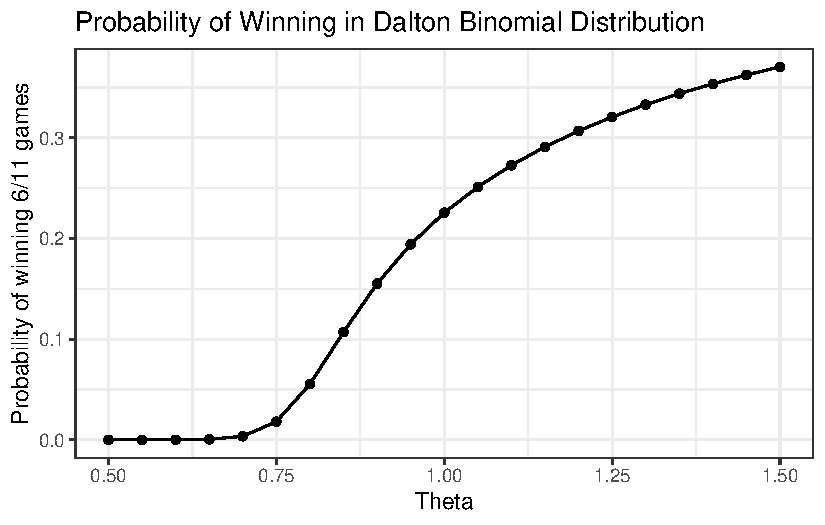
\includegraphics[keepaspectratio]{Lab10WriteUp_files/figure-pdf/unnamed-chunk-5-1.pdf}}

\normalsize

\subsection{Part b}\label{part-b}

Now, plot Altham's Multiplicative Binomial Distribution under the same
parameters with \(\theta=0.50\), \(\theta=1\), and \(\theta=1.5\). Use
\texttt{ncol=1} in \texttt{facet\_wrap()} to plot the PMFs in a single
column for comparing.

\normalsize

\begin{Shaded}
\begin{Highlighting}[numbers=left,,]
\NormalTok{ggdat }\OtherTok{\textless{}{-}} \FunctionTok{tibble}\NormalTok{(}\AttributeTok{x =}\NormalTok{ (}\DecValTok{0}\SpecialCharTok{:}\DecValTok{11}\NormalTok{)) }\SpecialCharTok{|\textgreater{}}
  \FunctionTok{mutate}\NormalTok{(}\AttributeTok{PMF05 =} \FunctionTok{daltbinom}\NormalTok{(}\AttributeTok{x =}\NormalTok{ x, }\AttributeTok{size =} \DecValTok{11}\NormalTok{, }\AttributeTok{prob =} \FloatTok{0.5}\NormalTok{, }\AttributeTok{theta =} \FloatTok{0.5}\NormalTok{)) }

\NormalTok{ggdat }\OtherTok{=}\NormalTok{ ggdat }\SpecialCharTok{|\textgreater{}}
       \FunctionTok{mutate}\NormalTok{(}\AttributeTok{PMF01 =} \FunctionTok{daltbinom}\NormalTok{(}\AttributeTok{x =}\NormalTok{ x, }\AttributeTok{size =} \DecValTok{11}\NormalTok{, }\AttributeTok{prob =} \FloatTok{0.5}\NormalTok{, }\AttributeTok{theta =} \DecValTok{1}\NormalTok{))}

\NormalTok{ggdat }\OtherTok{=}\NormalTok{ ggdat }\SpecialCharTok{|\textgreater{}}
      \FunctionTok{mutate}\NormalTok{(}\AttributeTok{PMF15 =} \FunctionTok{daltbinom}\NormalTok{(}\AttributeTok{x =}\NormalTok{ x, }\AttributeTok{size =} \DecValTok{11}\NormalTok{, }\AttributeTok{prob =} \FloatTok{0.5}\NormalTok{, }\AttributeTok{theta =} \FloatTok{1.5}\NormalTok{))}



\NormalTok{PMF05.plot }\OtherTok{\textless{}{-}} \FunctionTok{ggplot}\NormalTok{(ggdat) }\SpecialCharTok{+}
\FunctionTok{geom\_linerange}\NormalTok{(}\FunctionTok{aes}\NormalTok{(}\AttributeTok{x =}\NormalTok{ x, }\AttributeTok{ymin =} \DecValTok{0}\NormalTok{, }\AttributeTok{ymax =}\NormalTok{ PMF05)) }\SpecialCharTok{+}
\FunctionTok{geom\_linerange}\NormalTok{(}\AttributeTok{data =}\NormalTok{ ggdat }\SpecialCharTok{|\textgreater{}} \FunctionTok{filter}\NormalTok{(x}\SpecialCharTok{==}\DecValTok{2}\NormalTok{),}
\FunctionTok{aes}\NormalTok{(}\AttributeTok{x =}\NormalTok{ x, }\AttributeTok{ymin =} \DecValTok{0}\NormalTok{, }\AttributeTok{ymax =}\NormalTok{ PMF05)) }\SpecialCharTok{+}
\FunctionTok{geom\_hline}\NormalTok{(}\AttributeTok{yintercept =} \DecValTok{0}\NormalTok{) }\SpecialCharTok{+}
\FunctionTok{scale\_x\_continuous}\NormalTok{(}\StringTok{"P of Winning n games"}\NormalTok{,}
\AttributeTok{breaks =} \FunctionTok{seq}\NormalTok{(}\DecValTok{0}\NormalTok{, }\DecValTok{11}\NormalTok{, }\DecValTok{1}\NormalTok{)) }\SpecialCharTok{+}
\FunctionTok{ylab}\NormalTok{(}\StringTok{"Probability"}\NormalTok{) }\SpecialCharTok{+}
\FunctionTok{theme\_bw}\NormalTok{()}\SpecialCharTok{+}
\FunctionTok{ggtitle}\NormalTok{(}\StringTok{"Theta = 0.5"}\NormalTok{)}


\NormalTok{PMF01.plot }\OtherTok{\textless{}{-}} \FunctionTok{ggplot}\NormalTok{(ggdat) }\SpecialCharTok{+}
\FunctionTok{geom\_linerange}\NormalTok{(}\FunctionTok{aes}\NormalTok{(}\AttributeTok{x =}\NormalTok{ x, }\AttributeTok{ymin =} \DecValTok{0}\NormalTok{, }\AttributeTok{ymax =}\NormalTok{ PMF01)) }\SpecialCharTok{+}
\FunctionTok{geom\_linerange}\NormalTok{(}\AttributeTok{data =}\NormalTok{ ggdat }\SpecialCharTok{|\textgreater{}} \FunctionTok{filter}\NormalTok{(x}\SpecialCharTok{==}\DecValTok{2}\NormalTok{),}
\FunctionTok{aes}\NormalTok{(}\AttributeTok{x =}\NormalTok{ x, }\AttributeTok{ymin =} \DecValTok{0}\NormalTok{, }\AttributeTok{ymax =}\NormalTok{ PMF01)) }\SpecialCharTok{+}
\FunctionTok{geom\_hline}\NormalTok{(}\AttributeTok{yintercept =} \DecValTok{0}\NormalTok{) }\SpecialCharTok{+}
\FunctionTok{scale\_x\_continuous}\NormalTok{(}\StringTok{"P of Winning n games"}\NormalTok{,}
\AttributeTok{breaks =} \FunctionTok{seq}\NormalTok{(}\DecValTok{0}\NormalTok{, }\DecValTok{11}\NormalTok{, }\DecValTok{1}\NormalTok{)) }\SpecialCharTok{+}
\FunctionTok{ylab}\NormalTok{(}\StringTok{"Probability"}\NormalTok{) }\SpecialCharTok{+}
\FunctionTok{theme\_bw}\NormalTok{()}\SpecialCharTok{+}
\FunctionTok{ggtitle}\NormalTok{(}\StringTok{"Theta = 1"}\NormalTok{)}

\NormalTok{PMF15.plot }\OtherTok{\textless{}{-}} \FunctionTok{ggplot}\NormalTok{(ggdat) }\SpecialCharTok{+}
\FunctionTok{geom\_linerange}\NormalTok{(}\FunctionTok{aes}\NormalTok{(}\AttributeTok{x =}\NormalTok{ x, }\AttributeTok{ymin =} \DecValTok{0}\NormalTok{, }\AttributeTok{ymax =}\NormalTok{ PMF15)) }\SpecialCharTok{+}
\FunctionTok{geom\_linerange}\NormalTok{(}\AttributeTok{data =}\NormalTok{ ggdat }\SpecialCharTok{|\textgreater{}} \FunctionTok{filter}\NormalTok{(x}\SpecialCharTok{==}\DecValTok{2}\NormalTok{),}
\FunctionTok{aes}\NormalTok{(}\AttributeTok{x =}\NormalTok{ x, }\AttributeTok{ymin =} \DecValTok{0}\NormalTok{, }\AttributeTok{ymax =}\NormalTok{ PMF15)) }\SpecialCharTok{+}
\FunctionTok{geom\_hline}\NormalTok{(}\AttributeTok{yintercept =} \DecValTok{0}\NormalTok{) }\SpecialCharTok{+}
\FunctionTok{scale\_x\_continuous}\NormalTok{(}\StringTok{"P of Winning n games"}\NormalTok{,}
\AttributeTok{breaks =} \FunctionTok{seq}\NormalTok{(}\DecValTok{0}\NormalTok{, }\DecValTok{11}\NormalTok{, }\DecValTok{1}\NormalTok{)) }\SpecialCharTok{+}
\FunctionTok{ylab}\NormalTok{(}\StringTok{"Probability"}\NormalTok{) }\SpecialCharTok{+}
\FunctionTok{theme\_bw}\NormalTok{()}\SpecialCharTok{+}
\FunctionTok{ggtitle}\NormalTok{(}\StringTok{"Theta = 1"}\NormalTok{)}

\NormalTok{PMF05.plot }\SpecialCharTok{/}\NormalTok{ PMF01.plot }\SpecialCharTok{/}\NormalTok{ PMF15.plot}
\end{Highlighting}
\end{Shaded}

\pandocbounded{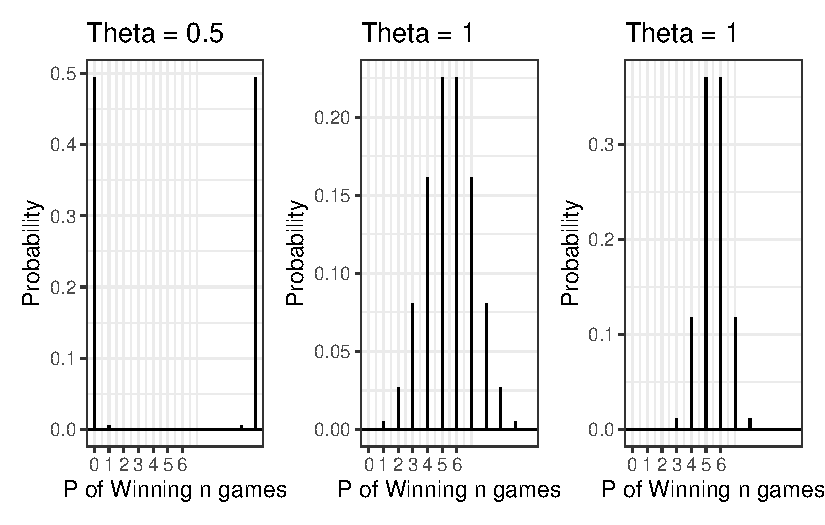
\includegraphics[keepaspectratio]{Lab10WriteUp_files/figure-pdf/unnamed-chunk-6-1.pdf}}

\normalsize

\subsection{Part c}\label{part-c}

What is your best assessment of what \(\theta\) is doing in this
setting. Consider when a 6-0 blowout is most likely, and when a 5-6
nail-biter is most likely. Note here we should treat the match as a
fixed \(n=11\) as we did for \(n=3\) in Lab 8.\\
\textbf{Note:} In lab 8, we saw that small \(\theta\) meant wins came in
bunches (clumped together), so there were more 2-0 wins in a best of
three series.

\textbf{Solution}

Here, we can see that theta is essentially a measure of how extreme the
values will be in a distribution. A low theta (\(<1\)) corresponds to an
expectation of extreme outcomes, and a high theta (\(>1\)) corrresponds
to an expectation of moederate values. Here, this is interpreted as us
expecting a close match, with both players winning a similar amount of
games, when theta is low. Similarly, we expect blowouts when theta is
high. When theta is moderate, we expect close-ish games, but accept that
there will be some blowouts. I think that theta \(\approx 1\) is the
most appropriate for this situation.

\section{Question 2}\label{question-2}

\subsection{Part a}\label{part-a-1}

Altham's Multiplicative Binomial Distribution does not typically
simplify to the clean \(E(X)=np\) seen in the Binomial distribution,
unless \(\theta = 1\). Write out the expression that would need to be
solved to find \(E(X^k)\), and then write a function that computes it
given the proposed parameter values \(p\) (\texttt{prob}) and \(\theta\)
(\texttt{theta}).

\textbf{Solution}

We have the formula for the \(k^{th}\) moment: \[
E(X) = \sum_{x= -\infty}^{\infty}xf_x(x)
\]

which we can compute here:

\normalsize

\begin{Shaded}
\begin{Highlighting}[numbers=left,,]
\CommentTok{\# Note that our PMF is 0 outside the range 0,11, so instead of computing over the integers we just use the integers in [0,11]. }
\NormalTok{Exk }\OtherTok{=} \ControlFlowTok{function}\NormalTok{(k, size, prob, theta)\{}
\NormalTok{  x }\OtherTok{=} \DecValTok{0}\SpecialCharTok{:}\NormalTok{size}
\NormalTok{  fx }\OtherTok{=} \FunctionTok{daltbinom}\NormalTok{(}\AttributeTok{x =}\NormalTok{ x, }\AttributeTok{size =}\NormalTok{ size, }\AttributeTok{prob =}\NormalTok{ prob, }\AttributeTok{theta =}\NormalTok{ theta)}
  \FunctionTok{return}\NormalTok{(}\FunctionTok{sum}\NormalTok{(x}\SpecialCharTok{\^{}}\NormalTok{k}\SpecialCharTok{*}\NormalTok{fx))}
\NormalTok{\}}

\FunctionTok{Exk}\NormalTok{(}\DecValTok{1}\NormalTok{, }\DecValTok{11}\NormalTok{, }\FloatTok{0.5}\NormalTok{, }\DecValTok{1}\NormalTok{)}
\end{Highlighting}
\end{Shaded}

\begin{verbatim}
[1] 5.5
\end{verbatim}

\begin{Shaded}
\begin{Highlighting}[numbers=left,,]
\NormalTok{n }\OtherTok{=} \DecValTok{11}
\NormalTok{p }\OtherTok{=} \FloatTok{0.5}

\NormalTok{(n}\SpecialCharTok{*}\NormalTok{p)}
\end{Highlighting}
\end{Shaded}

\begin{verbatim}
[1] 5.5
\end{verbatim}

\begin{Shaded}
\begin{Highlighting}[numbers=left,,]
\CommentTok{\# Our expected value of the altham binomial matches that of the binomial for theta = 1. }
\CommentTok{\# This makes sense, as the Altham distribution for theta = 1 is the binomial distribution.}
\end{Highlighting}
\end{Shaded}

\normalsize

\subsection{Part b}\label{part-b-1}

Describe how you can use your answer to part a to find Method of Moments
estimates for the parameters \(p\) and \(\theta\) for Altham's
Multiplicative Binomial Distribution based on data.

\textbf{Solution}

From a dataset, we can obtain a first and second moment. We set the
formula for the \(1st\) moment (which is a function that takes arguments
theta and p) equal to our observed value from the dataset. We do the
same for the second moment. We now have two equations and two unknowns,
and can use row reduction to solve for the two unknowns.

\subsection{Part c}\label{part-c-1}

Write a function that computes the log-likelihood for Altham's
Multiplicative Binomial Distribution, given data (\texttt{x}) and
proposed parameter values \(p\) (\texttt{prob}) and \(\theta\)
(\texttt{theta}).

\textbf{Solution}

\normalsize

\begin{Shaded}
\begin{Highlighting}[numbers=left,,]
\CommentTok{\# Let\textquotesingle{}s assume x is a dataframe or tibble with columns event \# and success. }
\CommentTok{\# }
\CommentTok{\# We could easily find n from the length of the "event" column vector, so we will write our function for arbitrary n}


\CommentTok{\# Let\textquotesingle{}s create an arbitrary x vector to test:}


\NormalTok{loglik }\OtherTok{=} \ControlFlowTok{function}\NormalTok{(x, size, p, theta)\{}
\NormalTok{   results }\OtherTok{=} \FunctionTok{daltbinom}\NormalTok{(}\AttributeTok{x =}\NormalTok{ x, }\AttributeTok{size =}\NormalTok{ size, }\AttributeTok{prob =}\NormalTok{ p, }\AttributeTok{theta =}\NormalTok{ theta)}
\NormalTok{   lik }\OtherTok{=}\NormalTok{ base}\SpecialCharTok{::}\FunctionTok{log}\NormalTok{(results)}
   \FunctionTok{return}\NormalTok{(}\FunctionTok{sum}\NormalTok{(lik))}
\NormalTok{  \}}

\CommentTok{\# Example scenario}

\NormalTok{x }\OtherTok{=} \FunctionTok{c}\NormalTok{(}\DecValTok{1}\NormalTok{,}\DecValTok{1}\NormalTok{,}\DecValTok{2}\NormalTok{,}\DecValTok{4}\NormalTok{,}\DecValTok{5}\NormalTok{,}\DecValTok{6}\NormalTok{,}\DecValTok{11}\NormalTok{,}\DecValTok{4}\NormalTok{,}\DecValTok{3}\NormalTok{,}\DecValTok{5}\NormalTok{,}\DecValTok{9}\NormalTok{,}\DecValTok{8}\NormalTok{,}\DecValTok{9}\NormalTok{,}\DecValTok{3}\NormalTok{,}\DecValTok{8}\NormalTok{,}\DecValTok{4}\NormalTok{,}\DecValTok{8}\NormalTok{,}\DecValTok{3}\NormalTok{,}\DecValTok{11}\NormalTok{,}\DecValTok{10}\NormalTok{,}\DecValTok{10}\NormalTok{,}\DecValTok{10}\NormalTok{,}\DecValTok{1}\NormalTok{,}\DecValTok{1}\NormalTok{,}\DecValTok{1}\NormalTok{,}\DecValTok{2}\NormalTok{,}\DecValTok{2}\NormalTok{,}\DecValTok{4}\NormalTok{,}\DecValTok{7}\NormalTok{,}\DecValTok{9}\NormalTok{,}\DecValTok{0}\NormalTok{,}\DecValTok{0}\NormalTok{,}\DecValTok{9}\NormalTok{,}\DecValTok{7}\NormalTok{,}\DecValTok{4}\NormalTok{)}

\FunctionTok{loglik}\NormalTok{(}\AttributeTok{x =}\NormalTok{ x, }\AttributeTok{size =} \DecValTok{11}\NormalTok{, }\AttributeTok{p =} \FloatTok{0.5}\NormalTok{, }\AttributeTok{theta =} \DecValTok{1}\NormalTok{)}
\end{Highlighting}
\end{Shaded}

\begin{verbatim}
[1] -129.9912
\end{verbatim}

\normalsize

\subsection{Part d}\label{part-d}

Describe how you can use your answer to part c to find Maximum
Likelihood estimates for the parameters \(p\) and \(\theta\) for
Altham's Multiplicative Binomial Distribution based on data.

\textbf{Solution}

We would use use calculus (via the \texttt{optim} function) to optimize
theta and p for the highest (least negative) value of the log-likelihood
function. We could plot result this using a color gradient, as we did in
class.

\section{Lab 10}\label{lab-10}

Peter ``Snakebite'' Wright is a two-time Professional Darts Corporation
World Champion (2020, 2022) and a former World No.~1. He is one of the
sport's most decorated players, winning nearly 50 PDC titles including
the World Matchplay, UK Open, and multiple European Championships.

In 2024, he made The Premier League -- a league involving the eight best
players that runs every Thursday night from February to May. In this
season, he won two of eighteen matches, securing only four points. The
spread in legs won was -43, meaning he lost 43 more legs than he won.
This performance was rather quite bad. He was soundly trounced in almost
all his match ups.

The 2024 standings are below:

\begin{longtable}[]{@{}ll@{}}
\toprule\noalign{}
Rank & Player \\
\midrule\noalign{}
\endhead
\bottomrule\noalign{}
\endlastfoot
1 & Luke Littler \\
2 & Luke Humphries \\
3 & Michael van Gerwen \\
4 & Michael Smith \\
5 & Nathan Aspinall \\
6 & Rob Cross \\
7 & Gerwyn Price \\
8 & Peter Wright \\
\end{longtable}

\subsection{Summarize the 2024 Data}\label{summarize-the-2024-data}

In \texttt{pdc2024.csv}, I have provided the data for the 2024 Premier
League season. There are a few data cleaning steps to consider.

\begin{itemize}
\tightlist
\item
  Remove any matches with no \texttt{Score} (e.g., a bye or walkover)
\item
  Nights 1 through 16 are best of 11 (first to 6), but the playoffs are
  extended. For consistency, keep nights 1 through 16 only.
\item
  Make two columns \texttt{WinnerLegs} and \texttt{LoserLegs} that keep
  track of the number of legs each player has won
\end{itemize}

Summarize the data. What do the data tell us about the breakdown of the
results?

\textbf{Solution}

\normalsize

\begin{Shaded}
\begin{Highlighting}[numbers=left,,]
\CommentTok{\# data cleaning:}

\NormalTok{dat.pdc }\OtherTok{=} \FunctionTok{read\_csv}\NormalTok{(}\StringTok{"pdc2024.csv"}\NormalTok{)}
\NormalTok{dat.pdc }\OtherTok{=} \FunctionTok{tibble}\NormalTok{(dat.pdc) }\SpecialCharTok{|\textgreater{}}
  \FunctionTok{filter}\NormalTok{(Score }\SpecialCharTok{!=} \StringTok{"w/o"}\NormalTok{) }\SpecialCharTok{|\textgreater{}}
  \FunctionTok{filter}\NormalTok{(Night }\SpecialCharTok{!=}  \StringTok{"Finals"}\NormalTok{) }\SpecialCharTok{|\textgreater{}}
  \FunctionTok{mutate}\NormalTok{(}\AttributeTok{Matchnum =} \FunctionTok{row\_number}\NormalTok{()) }\SpecialCharTok{|\textgreater{}}
  \FunctionTok{separate}\NormalTok{(Score, }\AttributeTok{into =} \FunctionTok{c}\NormalTok{(}\StringTok{"WinnerLegs"}\NormalTok{, }\StringTok{"LoserLegs"}\NormalTok{), }\AttributeTok{sep =} \StringTok{"{-}"}\NormalTok{, }\AttributeTok{convert =} \ConstantTok{TRUE}\NormalTok{)}
\end{Highlighting}
\end{Shaded}

\normalsize

\normalsize

\begin{Shaded}
\begin{Highlighting}[numbers=left,,]
\CommentTok{\# Failed attempts:}

\CommentTok{\# dat.pdc = read\_csv("pdc2024.csv")}
\CommentTok{\# dat.pdc = tibble(dat.pdc) |\textgreater{}}
\CommentTok{\#   filter(Score != "w/o") |\textgreater{}}
\CommentTok{\#   filter(Night !=  "Finals") |\textgreater{}}
\CommentTok{\#   mutate(Matchnum = row\_number()) |\textgreater{}}
\CommentTok{\#   separate(Score, into = c("WinnerLegs", "LoserLegs"), sep = "{-}", convert = TRUE) |\textgreater{}}
\CommentTok{\#   group\_by(Winner) |\textgreater{}}
\CommentTok{\#   arrange(Matchnum, .by\_group = TRUE) |\textgreater{}}
\CommentTok{\#   mutate(LegsWon = cumsum(WinnerLegs)) |\textgreater{}}
\CommentTok{\#   ungroup() |\textgreater{}}
\CommentTok{\#   arrange(Matchnum)}



\CommentTok{\# dat.pdc = read\_csv("pdc2024.csv")}

\CommentTok{\# \# function()}
\CommentTok{\# dat.pdc = tibble(dat.pdc) |\textgreater{}}
\CommentTok{\#   filter(Score != "w/o") |\textgreater{}}
\CommentTok{\#   filter(Night !=  "Finals") |\textgreater{}}
\CommentTok{\#   separate(Score, into = c("WinnerLegs", "LoserLegs"), sep = "{-}", convert = TRUE)}

\CommentTok{\# Legstat = function(player)\{}
\CommentTok{\#   dat.pdc = dat.pdc |\textgreater{}}
\CommentTok{\#   mutate(LegsWonLittler = LoserLegs * (Loser == Player)+ 6*(Winner == Player)) |\textgreater{}}
\CommentTok{\# \}}
\CommentTok{\# \# sapply(unique(players), dat.pdc)}

\CommentTok{\# dat.pdc = tibble(dat.pdc) |\textgreater{}}
\CommentTok{\#  filter(Winner == "Luke Littler" | Loser == "Luke Littler") |\textgreater{}}
\CommentTok{\#  mutate(Littler = case\_when(Winner == "Luke Littler" \textasciitilde{} 6, Loser == "Luke Littler" \textasciitilde{} LoserLegs)) |\textgreater{}}
\CommentTok{\#  mutate(LittlerWins = cumsum(Littler))}
\end{Highlighting}
\end{Shaded}

\normalsize

\normalsize

\begin{Shaded}
\begin{Highlighting}[numbers=left,,]
\NormalTok{dat.pdc }\OtherTok{=}\NormalTok{ dat.pdc }\SpecialCharTok{|\textgreater{}} \FunctionTok{mutate}\NormalTok{(}\AttributeTok{MatchID =} \FunctionTok{row\_number}\NormalTok{())}

\NormalTok{cum\_legs }\OtherTok{=} \ControlFlowTok{function}\NormalTok{(player) \{}
\NormalTok{  dat.pdc }\SpecialCharTok{|\textgreater{}}
    \FunctionTok{filter}\NormalTok{(Winner }\SpecialCharTok{==}\NormalTok{ player }\SpecialCharTok{|}\NormalTok{ Loser }\SpecialCharTok{==}\NormalTok{ player) }\SpecialCharTok{|\textgreater{}}
    \FunctionTok{mutate}\NormalTok{(}
      \AttributeTok{LegsWon =} \FunctionTok{case\_when}\NormalTok{(}
\NormalTok{        Winner }\SpecialCharTok{==}\NormalTok{ player }\SpecialCharTok{\textasciitilde{}}\NormalTok{ WinnerLegs,}
\NormalTok{        Loser  }\SpecialCharTok{==}\NormalTok{ player }\SpecialCharTok{\textasciitilde{}}\NormalTok{ LoserLegs}
\NormalTok{      ),}
      \AttributeTok{CumLegsWon =} \FunctionTok{cumsum}\NormalTok{(LegsWon)}
\NormalTok{    ) }\SpecialCharTok{|\textgreater{}}
    \FunctionTok{select}\NormalTok{(MatchID, CumLegsWon) }\SpecialCharTok{|\textgreater{}}
    \FunctionTok{rename}\NormalTok{(}\SpecialCharTok{!!}\AttributeTok{player :=}\NormalTok{ CumLegsWon)}
\NormalTok{\}}

\NormalTok{players }\OtherTok{=} \FunctionTok{unique}\NormalTok{(}\FunctionTok{as.character}\NormalTok{(}\FunctionTok{c}\NormalTok{(dat.pdc}\SpecialCharTok{$}\NormalTok{Winner, dat.pdc}\SpecialCharTok{$}\NormalTok{Loser)))}

\NormalTok{cum\_data }\OtherTok{=} \FunctionTok{map}\NormalTok{(players, cum\_legs) }\SpecialCharTok{|\textgreater{}} \FunctionTok{reduce}\NormalTok{(full\_join, }\AttributeTok{by =} \StringTok{"MatchID"}\NormalTok{)}

\NormalTok{dat.pdc }\OtherTok{=}\NormalTok{ dat.pdc }\SpecialCharTok{|\textgreater{}} \FunctionTok{left\_join}\NormalTok{(cum\_data, }\AttributeTok{by =} \StringTok{"MatchID"}\NormalTok{)}

\NormalTok{dat.pdc }\OtherTok{=}\NormalTok{ dat.pdc }\SpecialCharTok{|\textgreater{}}
  \FunctionTok{fill}\NormalTok{(}\FunctionTok{any\_of}\NormalTok{(players), }\AttributeTok{.direction =} \StringTok{"down"}\NormalTok{) }\SpecialCharTok{|\textgreater{}}
  \FunctionTok{mutate}\NormalTok{(}\FunctionTok{across}\NormalTok{(}\FunctionTok{any\_of}\NormalTok{(players), }\SpecialCharTok{\textasciitilde{}} \FunctionTok{replace\_na}\NormalTok{(., }\DecValTok{0}\NormalTok{)))}
\end{Highlighting}
\end{Shaded}

\normalsize

\normalsize

\begin{Shaded}
\begin{Highlighting}[numbers=left,,]
\NormalTok{dat.pdc }\SpecialCharTok{|\textgreater{}}
  \FunctionTok{pivot\_longer}\NormalTok{(}\FunctionTok{any\_of}\NormalTok{(players), }\AttributeTok{names\_to =} \StringTok{"Player"}\NormalTok{, }\AttributeTok{values\_to =} \StringTok{"CumLegs"}\NormalTok{) }\SpecialCharTok{|\textgreater{}}
  \FunctionTok{filter}\NormalTok{(}\SpecialCharTok{!}\FunctionTok{is.na}\NormalTok{(CumLegs)) }\SpecialCharTok{|\textgreater{}}
  \FunctionTok{ggplot}\NormalTok{(}\FunctionTok{aes}\NormalTok{(}\AttributeTok{x =}\NormalTok{ MatchID, }\AttributeTok{y =}\NormalTok{ CumLegs, }\AttributeTok{color =}\NormalTok{ Player)) }\SpecialCharTok{+}
  \FunctionTok{geom\_line}\NormalTok{() }\SpecialCharTok{+}
  \FunctionTok{labs}\NormalTok{(}\AttributeTok{x =} \StringTok{"Games Played"}\NormalTok{, }\AttributeTok{y =} \StringTok{"Cumulative Legs Won"}\NormalTok{, }\AttributeTok{color =} \StringTok{"Player"}\NormalTok{) }\SpecialCharTok{+}
  \FunctionTok{theme\_minimal}\NormalTok{()}
\end{Highlighting}
\end{Shaded}

\pandocbounded{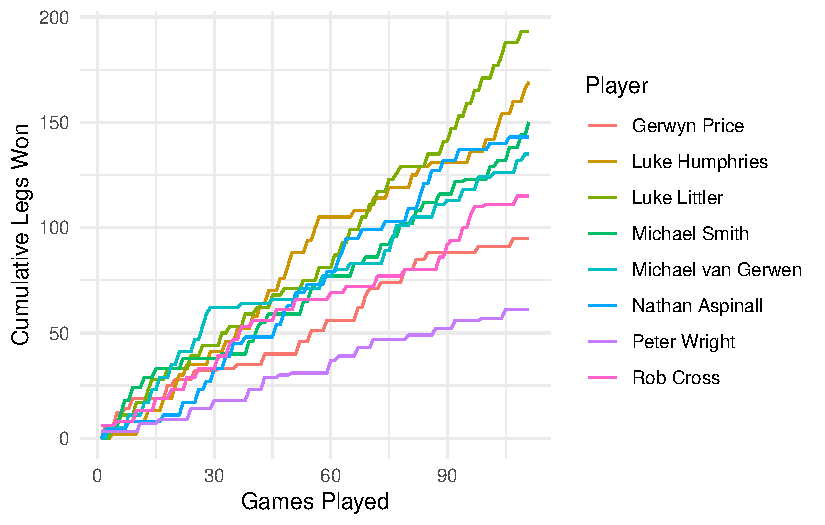
\includegraphics[keepaspectratio]{Lab10WriteUp_files/figure-pdf/unnamed-chunk-12-1.pdf}}

\begin{Shaded}
\begin{Highlighting}[numbers=left,,]
\CommentTok{\#I had to look up a lot of functions to make this plot and the data manipulation possible. If there is an easier solution I would be very interested to see it, but I tried to do it simply for a while and couldn\textquotesingle{}t find anything super elegant.}
\end{Highlighting}
\end{Shaded}

\normalsize

From this plot, the way that the season evolved, for each player and as
a league, is clear. Some notable trends are:

\begin{itemize}
\tightlist
\item
  Luke Littler's surge in the last quarter of the season
\item
  Peter Wright's consistently poor performance
\item
  The mid-season reign of Luke Humphries
\item
  After the first 30 games, there were only three leaders, two of which
  finished first and second. Michael van Gerwen had a short stint of
  domination in the early season, but faded to a mediocre finish by the
  end.
\end{itemize}

\subsection{Altham's Multiplicative Binomial
Distribution}\label{althams-multiplicative-binomial-distribution-1}

For each player in the 2024 season, use the number of legs won in each
match to compute maximium likelihood estimates for \(p\) and
\(\theta\).\\
\textbf{Note}: The ``for each'' here can be done more efficiently with a
function or a loop!

\begin{itemize}
\tightlist
\item
  Create a vector containing the number of legs won by the player. Note
  sometimes you will need to pull from winner's legs and sometimes from
  the loser's legs.
\item
  Find the MLE for the player using this data. Ensure to report \(p\)
  and \(\theta\) for each player in a nicely formatted table.\\
  \textbf{Note:} In Lecture on Monday, we used transformations to
  restrict how \texttt{optim()} searches the parameter space. For
  example, here, you might consider
  \texttt{p\ \textless{}-\ 1/(1+exp(-par{[}1{]}))} and
  \texttt{theta\ \textless{}-\ exp(par{[}2{]})}.
\item
  Make comments about the MLEs in the context of the standings.
\end{itemize}

\textbf{Solution}

\normalsize

\begin{Shaded}
\begin{Highlighting}[numbers=left,,]
\NormalTok{legs }\OtherTok{=} \ControlFlowTok{function}\NormalTok{(player) \{}
\NormalTok{  dat.pdc }\SpecialCharTok{|\textgreater{}}
    \FunctionTok{filter}\NormalTok{(Winner }\SpecialCharTok{==}\NormalTok{ player }\SpecialCharTok{|}\NormalTok{ Loser }\SpecialCharTok{==}\NormalTok{ player) }\SpecialCharTok{|\textgreater{}}
    \FunctionTok{mutate}\NormalTok{(}
      \AttributeTok{LegsWon =} \FunctionTok{case\_when}\NormalTok{(}
\NormalTok{        Winner }\SpecialCharTok{==}\NormalTok{ player }\SpecialCharTok{\textasciitilde{}}\NormalTok{ WinnerLegs,}
\NormalTok{        Loser  }\SpecialCharTok{==}\NormalTok{ player }\SpecialCharTok{\textasciitilde{}}\NormalTok{ LoserLegs}
\NormalTok{      )}
\NormalTok{    ) }\SpecialCharTok{|\textgreater{}}
    \FunctionTok{select}\NormalTok{(MatchID, LegsWon) }\SpecialCharTok{|\textgreater{}}
    \FunctionTok{rename}\NormalTok{(}\SpecialCharTok{!!}\FunctionTok{paste0}\NormalTok{(player, }\StringTok{"\_dist"}\NormalTok{) }\SpecialCharTok{:}\ErrorTok{=}\NormalTok{ LegsWon)}
\NormalTok{\}}
 \CommentTok{\#paste0 so there are no spaces, needed to distinguish these columns from cumulative columns}

\NormalTok{legs\_data }\OtherTok{=} \FunctionTok{map}\NormalTok{(players, legs) }\SpecialCharTok{|\textgreater{}} \FunctionTok{reduce}\NormalTok{(full\_join, }\AttributeTok{by =} \StringTok{"MatchID"}\NormalTok{)}

\NormalTok{dat.pdc }\OtherTok{=}\NormalTok{ dat.pdc }\SpecialCharTok{|\textgreater{}} \FunctionTok{left\_join}\NormalTok{(legs\_data, }\AttributeTok{by =} \StringTok{"MatchID"}\NormalTok{)}
\end{Highlighting}
\end{Shaded}

\normalsize

\normalsize

\begin{Shaded}
\begin{Highlighting}[numbers=left,,]
\NormalTok{altham\_mle }\OtherTok{=} \ControlFlowTok{function}\NormalTok{(player) \{}
\NormalTok{  y }\OtherTok{=}\NormalTok{ dat.pdc }\SpecialCharTok{|\textgreater{}}
    \FunctionTok{filter}\NormalTok{(}\SpecialCharTok{!}\FunctionTok{is.na}\NormalTok{(}\SpecialCharTok{!!}\FunctionTok{sym}\NormalTok{(}\FunctionTok{paste0}\NormalTok{(player, }\StringTok{"\_dist"}\NormalTok{)))) }\SpecialCharTok{|\textgreater{}}
    \FunctionTok{pull}\NormalTok{(}\SpecialCharTok{!!}\FunctionTok{sym}\NormalTok{(}\FunctionTok{paste0}\NormalTok{(player, }\StringTok{"\_dist"}\NormalTok{)))}
  
\NormalTok{  nll }\OtherTok{=} \ControlFlowTok{function}\NormalTok{(par) \{}
\NormalTok{    p     }\OtherTok{=} \DecValTok{1} \SpecialCharTok{/}\NormalTok{ (}\DecValTok{1} \SpecialCharTok{+} \FunctionTok{exp}\NormalTok{(}\SpecialCharTok{{-}}\NormalTok{par[}\DecValTok{1}\NormalTok{]))}
\NormalTok{    theta }\OtherTok{=} \FunctionTok{exp}\NormalTok{(par[}\DecValTok{2}\NormalTok{])}
    \SpecialCharTok{{-}}\FunctionTok{loglik}\NormalTok{(}\AttributeTok{x =}\NormalTok{ y, }\AttributeTok{size =} \DecValTok{11}\NormalTok{, }\AttributeTok{p =}\NormalTok{ p, }\AttributeTok{theta =}\NormalTok{ theta)}
\NormalTok{  \}}
  
\NormalTok{  fit }\OtherTok{=} \FunctionTok{optim}\NormalTok{(}\FunctionTok{c}\NormalTok{(}\DecValTok{0}\NormalTok{, }\DecValTok{0}\NormalTok{), nll)}
  
  \FunctionTok{tibble}\NormalTok{(}
    \AttributeTok{Player =}\NormalTok{ player,}
    \AttributeTok{p      =} \DecValTok{1} \SpecialCharTok{/}\NormalTok{ (}\DecValTok{1} \SpecialCharTok{+} \FunctionTok{exp}\NormalTok{(}\SpecialCharTok{{-}}\NormalTok{fit}\SpecialCharTok{$}\NormalTok{par[}\DecValTok{1}\NormalTok{])),}
    \AttributeTok{theta  =} \FunctionTok{exp}\NormalTok{(fit}\SpecialCharTok{$}\NormalTok{par[}\DecValTok{2}\NormalTok{])}
\NormalTok{  )}
\NormalTok{\}}

\NormalTok{rank\_order }\OtherTok{=} \FunctionTok{tibble}\NormalTok{(}
  \AttributeTok{Player =} \FunctionTok{c}\NormalTok{(}\StringTok{"Luke Littler"}\NormalTok{, }\StringTok{"Luke Humphries"}\NormalTok{, }\StringTok{"Michael van Gerwen"}\NormalTok{, }\StringTok{"Michael Smith"}\NormalTok{, }\StringTok{"Nathan Aspinall"}\NormalTok{, }\StringTok{"Rob Cross"}\NormalTok{,}
  \StringTok{"Gerwyn Price"}\NormalTok{, }\StringTok{"Peter Wright"}\NormalTok{),}
  \AttributeTok{Rank =} \DecValTok{1}\SpecialCharTok{:}\DecValTok{8}
\NormalTok{)}

\NormalTok{mle\_table }\OtherTok{=} \FunctionTok{map}\NormalTok{(players, altham\_mle) }\SpecialCharTok{|\textgreater{}} \FunctionTok{list\_rbind}\NormalTok{() }\SpecialCharTok{|\textgreater{}}
  \FunctionTok{left\_join}\NormalTok{(rank\_order, }\AttributeTok{by =} \StringTok{"Player"}\NormalTok{) }\SpecialCharTok{|\textgreater{}}
  \FunctionTok{arrange}\NormalTok{(Rank) }\SpecialCharTok{|\textgreater{}}
  \FunctionTok{select}\NormalTok{(Rank, Player, p, theta)}

\NormalTok{knitr}\SpecialCharTok{::}\FunctionTok{kable}\NormalTok{(mle\_table, }\AttributeTok{digits =} \DecValTok{3}\NormalTok{,}
             \AttributeTok{caption =} \StringTok{"MLE Estimates for Altham\textquotesingle{}s Multiplicative Binomial Distribution"}\NormalTok{)}
\end{Highlighting}
\end{Shaded}

\begin{longtable}[]{@{}rlrr@{}}
\caption{MLE Estimates for Altham's Multiplicative Binomial
Distribution}\tabularnewline
\toprule\noalign{}
Rank & Player & p & theta \\
\midrule\noalign{}
\endfirsthead
\toprule\noalign{}
Rank & Player & p & theta \\
\midrule\noalign{}
\endhead
\bottomrule\noalign{}
\endlastfoot
1 & Luke Littler & 0.469 & 1.316 \\
2 & Luke Humphries & 0.461 & 1.205 \\
3 & Michael van Gerwen & 0.431 & 1.023 \\
4 & Michael Smith & 0.426 & 1.047 \\
5 & Nathan Aspinall & 0.403 & 1.186 \\
6 & Rob Cross & 0.395 & 1.014 \\
7 & Gerwyn Price & 0.383 & 1.020 \\
8 & Peter Wright & 0.317 & 0.989 \\
\end{longtable}

\normalsize

We get a result that corroborates what we know about distributions and
darts. The table, when ranked in order of final standings, is also
ranked from highest p (of winning one leg) to lowest. This means that
the players with the highest probabilities of winning a leg, have won
the most matches. This isn't necessarily surprising (actually, it would
be cool to run an analysis to see how suprising it actually is under
these conditions), but it also isn't guaranteed. We also see a (less
solid) positive correlation with theta and final standings. This is
interesting, and makes sense- winning more legs closer to each other
means that you're not spreading out your legs won between matches,
you're winning 6 instead of 5 times, for example. In theory, we could
have a player who won 5 games each match, which would have broken the
pattern we see here.

\subsection{Altham's Multiplicative Beta Binomial
Distribution}\label{althams-multiplicative-beta-binomial-distribution-1}

For each player in the 2024 season, use the number of legs won in each
match to compute maxmium likelihood estimates for \(p\) and
\(\theta\).\\
\textbf{Note}: The ``for each'' here can be done more efficiently with a
function or a loop!

\begin{itemize}
\tightlist
\item
  Create a vector containing the number of legs won by the player. Note
  sometimes you will need to pull from winner's legs and sometimes from
  the loser's legs.
\item
  Find the MLEs for the player using this data. Ensure to report
  \(\alpha\), \(\beta\), and \(\theta\) for each player in a nicely
  formatted table.\\
  \textbf{Note 1}: Due to the computational complexity of
  \texttt{integrate()}, you should compute the logged probability for
  \texttt{0:6} once and add them according to the data in each player's
  vector. \textbf{Note 2}: In Lecture on Monday, we used transformations
  to restrict how \texttt{optim()} searches the parameter space.
\item
  Plot the underlying Beta(\(\alpha\), \(\beta\)) distribution for each
  player.\\
  \textbf{Note}: Add the mean and variance of the Beta to the table of
  MLEs. Recall \begin{align*}
   E(X)   &= \frac{\alpha}{\alpha+\beta}\\
   sd(X) &= \sqrt{\frac{\alpha\beta}{(\alpha+\beta)^2(\alpha+\beta+1)}}
  \end{align*}
\item
  Make comments about the MLEs in the context of the standings.\\
  \textbf{Note}: The players alternate who throws first in a leg has the
  mathematical ``head start'' to reach a finish before their opponent
  can take another turn. Players alternate who throws first with each
  leg.
\end{itemize}

\subsection{Executive Summary}\label{executive-summary}

Summarize the work you've done here to provide a brief (200-300 word)
data-driven summary of the 2024 Premier League season using your work in
Lab 10. Your summary should be professional, clear, and all claims
should be corroborated with statistical support.




\end{document}
